 \begin{figure}
      \centering
      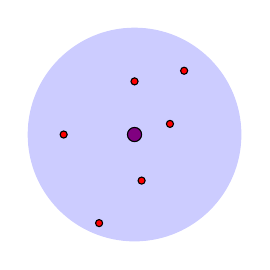
\begin{tikzpicture}[scale=0.45]
        \draw[blue!20, fill=blue!20] (3, 3) circle (3);
        \draw[fill=violet] (3,3) circle (0.2);
        \draw[fill=red] (3,4.5) circle (0.1);
        \draw[fill=red] (3.2,1.7) circle (0.1);
        \draw[fill=red] (1,3) circle (0.1);
        \draw[fill=red] (2,0.5) circle (0.1);
        \draw[fill=red] (4,3.3) circle (0.1);
        \draw[fill=red] (4.4,4.8) circle (0.1);
      \end{tikzpicture}
      \caption{\scriptsize{The observation preimage set $H(y)$ (circle). Any states
          in this region (red points) can get observation of the landmark $y$
          (violet point).}}
    \end{figure}